\chapter{Emulation and Monitoring of the Upstream Tracker RAW data}
\label{chapter:tbut}

This chapter is dedicated to present the emulation and monitoring tool for Upstream Tracker called TbUT.
To provide a full picture of the data emulation process, this chapter starts by introducing the physics principles of data collection. Within this section, the interaction of particles with matter and review of the principles of particle detection in silicon will be discussed.    
The TbUT tool was designed to emulate all raw data processing algorithms, as well as generate a number of performance plots. This software was implemented in order to process all raw data collected during the UT testbeams. The described software will also play a crucial role in the future monitoring and calibration of the UT detector. The outcome of this software will help to ensure the quality of the collected data. 


\section{Interaction of Particles with Matter}
\label{sec:Interaction}
When charged particle traverse through matter, it interacts with the material and loses its energy. The energy deposition is caused mostly by inelastic collisions with atomic electrons and elastic scattering from the nuclei of the absorbing material along the particle trajectory. For particles which masses are well above the mass of an electron the mean loss of energy is described by the Bethe-Bloch-Formula: 

\begin{equation}
\label{eq:Bethe_bloh}
  -\left< \frac{dE}{dx} \right> = K z^2 \frac{1}{\beta^2} \frac{Z}{A} 
  \left[ \frac{1}{2} \ln \frac{2m_e c^2 \beta^2 \gamma^2 T_{max}}{I^2} - \beta^2 - \frac{\delta(\beta \gamma)}{2}
  \right]  
\end{equation}

where: 
\begin{itemize}
    \item $\frac{dE}{dx}$ is energy loss of the particle usually given in $\frac{eV}{g/cm^{2}}$
    \item $K$ is a constant: $0.307~ MeV~ mol^{-1}~ cm^2$;
    \item $Z$ and $A$ are the atomic number and mass (for silicon 14 and 28 respectively);
    \item $c$ is the speed of light in vacuum;
    \item $\gamma = \frac{1}{\sqrt{1-\beta^2}}$ is the Lorenz Factor and $\beta = \frac{v}{c}$;
    \item $I$ is a medium average ionisation energy;
    \item $\delta(\beta \gamma)$ describes the density effect correction for high energy particles; 
    \item $T_{max}$ is the maximum energy transferred to a free electron in a single collision, given by:
    \begin{equation}
        T_{max} = \frac{2m_e c^2 \beta^2 \gamma^2}{1+2\gamma \frac{m_e}{M}+ (\frac{me}{M})^2}
    \end{equation}
\end{itemize}

The initial version of formula \ref{eq:Bethe_bloh} was proposed by Bethe \cite{Bethe} only three years after Schrodinger postulated non-relativistic Quantum Mechanic. The quantity $-\left< \frac{dE}{dx} \right>$ that is be calculated using this formula can be interpreted as stopping power of a particular material. Figure \ref{fig:Bethe_bloh} presents the stopping power for positive muons in copper as a function of $\beta \gamma$. 

For low energies term $\frac{1}{\beta^2}$ in equation \ref{eq:Bethe_bloh} is dominant and the stopping power decreases with increasing energy, reaching minimum when $(\beta \gamma) \approx 3 $. A particle with an energy loss at the mimimum is called a Minimum Ionizing Particle (MIP). 



\begin{figure}[h]
\centering
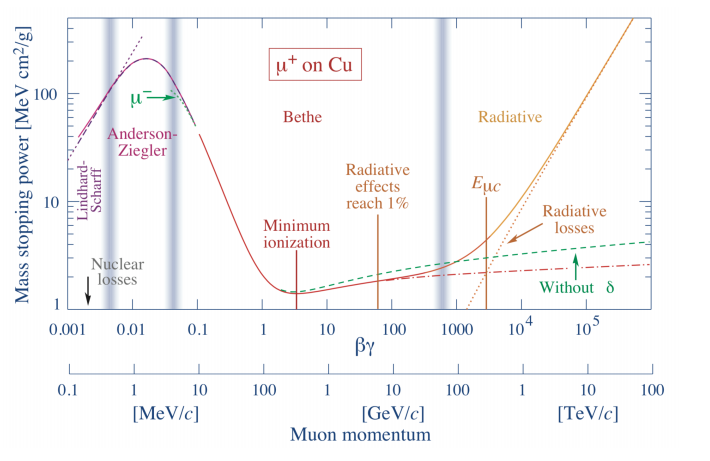
\includegraphics{figures/Bete_bloh.PNG}
\caption{ The stopping power $-\left< \frac{dE}{dx} \right>$ as a function of $\beta \gamma$. The region that the Bethe-Bloch formula describes is $0.1 \le (\beta \gamma) \le 1000$ and is highlighted in red. Figure taken from \cite{PDG}.
\label{fig:event display}}
\end{figure}


It is worth noticing that for a charged particle traversing a material, the number of collisions occurring and the amount of energy transferred in each collision is subject to statistical fluctuations. Formula \ref{eq:Bethe_bloh} provides only the average value of energy loss, which due to the statistical nature of the process, may vary from the actual value. 
For a relatively thick material, the number of collisions will be large enough to justify modeling distribution of the energy loss by the Gaussian \cite{gauss_sensor}. Although for a thinner materials, which are widely used in the current tracking detector, the average energy loss is small, so the large fluctuation in the deposited energy can be observed.    
 This results in a largely asymmetric charge distribution, which can be parametrized by the long-tailed Landau distribution shown in figure \ref{fig:}.  This distribution is traditionally fit with a Landau convoluted with a Gaussian to extract the peak charge collection, the Most Probable Value (MPV). The Landau-Gauss convolution is given by:

\begin{equation}
    \begin{split}
    f(x) = \frac{1}{\sqrt{2 \pi}} \frac{\tau}{\sigma_{noise} \sigma_{width}} \int_{x_0+5\sigma}^{x_0-5\sigma} Landau(x, \tau, \sigma_{width}) \\ \times Gauss (x, x_0,\sigma_{noise}) dx
    \end{split}
\end{equation}

where :
\begin{equation}
    Landau(x,\tau) =  \frac{1}{\pi \tau} \int_{0}^{\infty} e^{-t \ln t - \frac{t \cdot x}{\tau}} \sin{\pi t} dt
\end{equation}
and $\tau$ is a Landau Most Provable Value (MPV), $\sigma_{width}$ is a width of a Landau distribution and $\sigma_{noise}$ is a Gaussian standard deviation. Landau Gauss convolution is calculated using numerical integration. 


\section{Operational principles of silicon detectors}

As described in chapter 1, a number of technologies are used for full event reconstruction at LHCb.  However, to achieve the highest precision and resolution, semiconducting detectors are currently the best option, since that kind of detector uses a minimal amount of material which particles need to traverse in order to be detected.  The only limitation of using this technology is its cost. Therefore they are placed where the highest resolution is required, such as around the interaction point in the LHCb detector. 
Most of the semiconducting detectors are made of silicon.  This is due to the fact that silicon is the second most abundant element on Earth as well as it is widely used in industrial applications. Silicon has an atomic number of 14, so it has 14 electrons in three shells (2,8,4 arrangement). The electrons arranged in the outer shell are the valence electrons.  Due to this electron arrangement, within the crystalline lattice structure, each silicon atom is surrounded by four neighbors, see figure \ref{fig:silicon}.  

\begin{figure}[h]
\centering
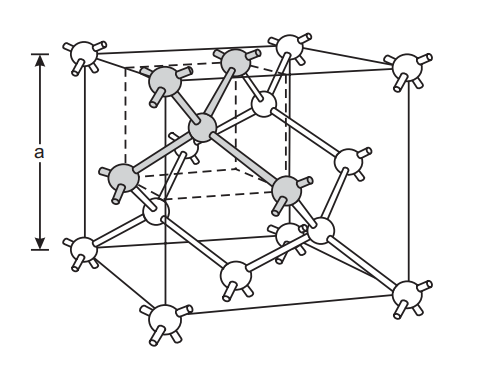
\includegraphics{figures/silicon.PNG}
\caption{Lattice structure of silicon. The building block of the lattice is formed by a central atom bonded to four
equidistant neighbors (indicated in gray). Figure taken from \cite{semiconductors_det_sys}}
\label{fig:silicon}
\end{figure}




The periodic potential of the crystalline structure results in the formation of electron energy bands. The energy bounds can be interpreted as a collection of the individual energy levels of electrons surrounding each atom. The wavefunctions of the individual electrons are overlapped with those of electrons enclosed to neighboring atoms, and due to the Pauli exclusion principle, the electron energy levels are prohibited from being the same so that one obtains a set of closely spaced energy levels, forming an energy band. 

At a temperature of absolute zero, the highest energy electrons lie in the valence band. Those electrons are strongly bonded to the atoms and thus are not able to carry the charge.  However, at the higher temperatures, electrons also occupy higher energy states known as the conduction band. The energy between the valence and conduction bands is called the band gap energy $E_g$.  The value of the band gap allows classifying materials into conductors, semiconductors, and insulators, which is shown in figure \ref{fig:boundgap}. 


\begin{figure}[h]
\centering
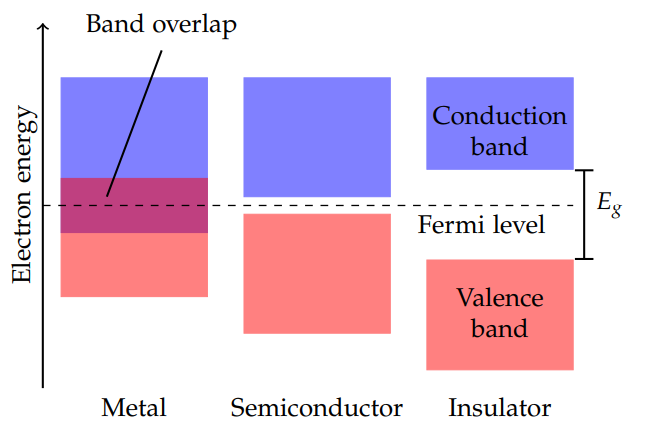
\includegraphics[scale=0.7]{figures/bound_gap.PNG}
\caption{Classification of metals, semiconductors and insulators according to their
band gap energy $E_g$. The Fermi level, denoted by the dashed line, is a hypothetical energy level which would have a 50\% probability of being occupied at thermal equilibrium.  Figure adapted from \cite{radiation_damage}}
\label{fig:boundgap}
\end{figure}

One of the most important features of semiconductors is their ability to change electrical conductivity by the introduction of impurity atoms, called dopants. These dopants replace atoms of the original material at lattice sites, and typically have more ($n$-type donors) or fewer ($p$-type donors) valence electrons in their outer shell, depending on the specific type of dopant. 


Most semiconductor detectors are made of $p-n$ junction, which manifests a diode characteristic. Such a semiconducting device is created by connecting two components of opposite dopping in good thermodynamical contact. The most important property of such a device is the phenomena of electrons diffusing into the $p$ region and holes into the $n$ region where they recombined. As a consequence, an electric field gradient is created, which eventually stops the diffusion process and establishes thermal equilibrium. Due to the electric field, there is a potential difference across the junction. The region of changing potential is known as depletion zone since it is almost fully depleted of all mobile charge carriers. This characteristic can be utilized for radiation detectors. Electron-hole pairs that are generated in the depletion zone by ionizing radiation will be separated by the electric field and can be detected if electrical contacts are connected to the device.


\section{TbUT Emulation Software}
The TbUT package is a software developed entirely by the author, and similarly to all of the official LHCb software, it is based on the Gaudi framework \cite{gaudi}. Gaudi identifies components with specific purposes and well-defined interfaces, interacting with each other to provide the complete functionality of an application. Gaudi provides to the application general-purpose components, like messaging and configuration services, see figure \ref{fig:gaudi flow}. The configuration is performed via the customized python scripts. By design, the Gaudi framework decouples objects describing data from those describing algorithms.



\begin{figure}[h]
\centering
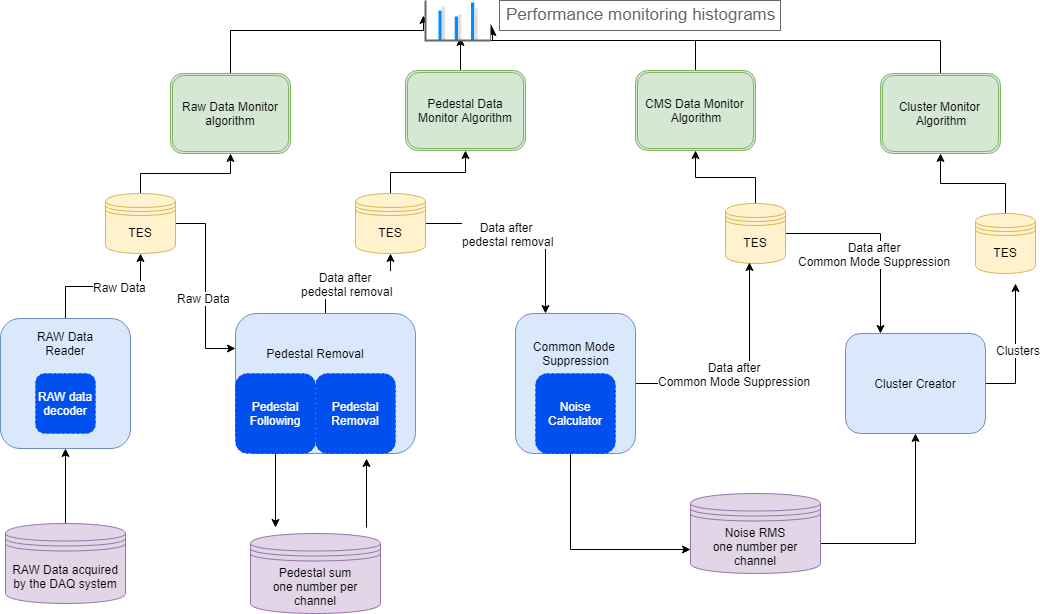
\includegraphics{figures/TBUT.png}
\caption{The diagram presenting the main component of the TbUT package and interactions between them. The light blue components are algorithms, dark blue is tools, and the violet ones represent serializable data. The direction of the arrows indicates whether the data is an input or output to the algorithm. }
\label{fig:TbUT}
\end{figure}


The software was designed based on the Object-oriented Programming paradigm.   This paradigm states that the software design is focused on data (also called \textbf{object}) rather than functions. An object can be defined as a data field that has unique attributes and behavior \cite{programming_paradigma}. 

Each of the TbUT components inherits from one of the following classes:  

\begin{itemize}
    \item \textbf{Algorithms}, these objects inherit from \textit{Gaudi::algorithm}, which is an essential part of the Gaudi application. They can read the input data, and via an appropriate tool process, they are able to generate the monitoring plots and store the data for the next processing steps. 
    \item \textbf{Monitoring algorithm}, these object, similarly to the \textbf{Algorithms}, inherit from  \textit{Gaudi::algorithm}. Their job is to extract data from TES and generate a set of monitoring histograms, which suppose to give an ultimate answer to the performance of the sensor. This component is key to make a  proper calibration. 
    \item \textbf{Tools} These objects inherit from the pure virtual interface \textit{IProcessingEngine}, and they were designed to perform the processing actions, for instance, pedestal removal. Figure \ref{fig:gaudi flow} presents the main components of the Gaudi framework.   
    \item \textbf{Serializable data} this objects inherits from the \textit{GaudiKernel::DataObject} are the result of the processing via the \textbf{Tools} and can be stored inside the Transient Event Store (TES). 
    \item \textbf{ Tool's Factories} these types of objects were implemented to create tools dynamically. Its concept was introduced in the Design Pattern book \cite{DesignPatterns}. 
\end{itemize}

\begin{figure}[h]
\centering
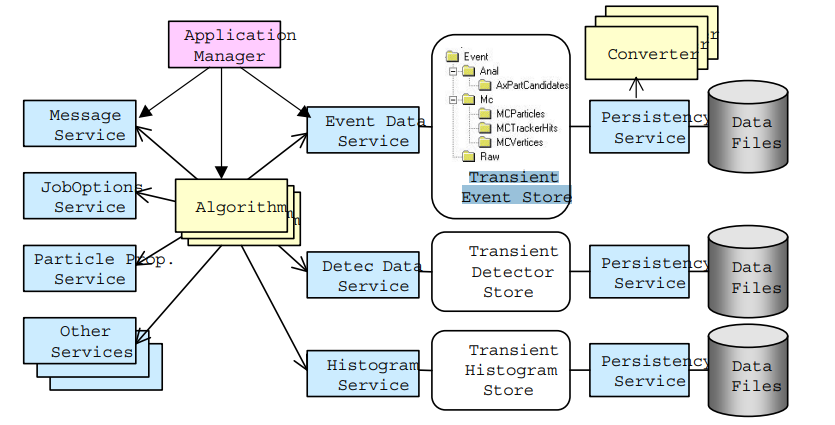
\includegraphics{figures/Gaudi.png}
\caption{Object Diagram of the Gaudi architecture, figure taken from \cite{Gaudi}}
\label{fig:gaudi flow}
\end{figure}


The first algorithm within the TbUT is dedicated to decoding the raw data acquired by the acquisition board, which is visualized in figure \ref{fig:TbUT}.  
During the lifetime of this project, the software has to able to process data acquired by the number of different DAQ systems, each of these producing the data in a completely different format.  To achieve that kind of flexibility the tool, that is responsible for reading the input data was implemented using a Factory Design Pattern \cite{DesignPatterns}. 

\subsection{Pedestal Subtraction}

Pedestals are the charge values measured by the read-out system in the absence of signal and noise. Each of the read-out channels can have a different ADC value of pedestal, and each pedestal's value depends on such environmental conditions as temperature, humidity, and operating conditions, like applied bias voltage. 
To ensure proper pedestals are removed from the raw ADC data, prior to each data collection run, the non-signal measurements (pedestal runs) are taken. Usually, pedestal data are quick to collect since no trigger is required. 

The pedestal subtraction algorithm has two phases. In first, the pedestal values are calculated. During the second one, the determined pedestal values are subtracted from the raw ADC data. Figure \ref{fig:ped} presents Pedestal Subtraction algorithm sequence diagram. That kind of UML diagram \cite{UML} is dedicated to depicts an interaction between objects in sequential order. These diagrams are widely used by businessmen and software developers to document and understand requirements for new and existing systems. 

\begin{figure}
\centering
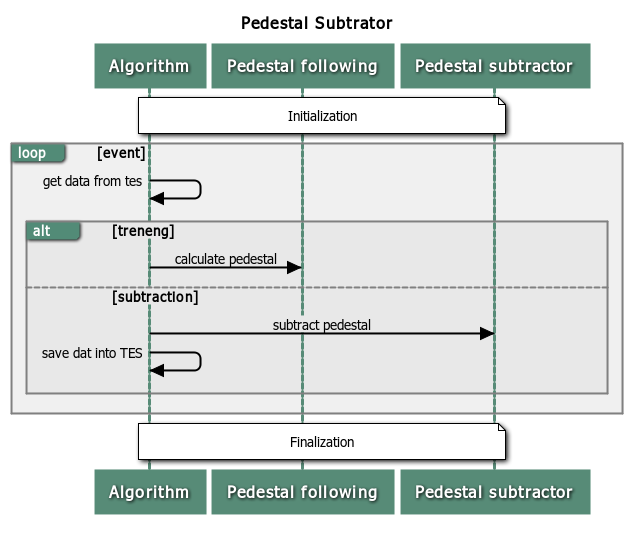
\includegraphics[scale=0.6]{figures/Pedestal_Subtrator.png}
\caption{Pedestal Subtraction sequence diagram.}
\label{fig:ped}
\end{figure}



\subsubsection{Pedestal following}
From the mathematical point of view the calculation of the pedestal is a running average. In every training event then pedestal sum is updated. This update takes into account the previously calculated value of the pedestal sum and the current ADC count. The pedestal sum is calculated for each channel separately. To be more precisely, the pedestal sum, $p^{sum}_i(n)$, for channel $i$ and event $n$ can be expressed as follows:

\begin{equation}
P_{i}^{sum}(n+1)=P^{sum}_{i}(n) + \frac{\Delta_{i}(n+1)}{N}
\label{eq:ped}
\end{equation}
Where the $\Delta_{i}(n+1)$ is a event to pedestal correction. This correction is expressed as:
\begin{equation}
\Delta_{i}(n+1)=ADC_{i}(n+1)-P^{sum}_{i}(n)
\end{equation}
In the equation \ref{eq:ped}, the $N$ is the weighting factor set by default to 1024. 


To increase the suitability of the pedestal, and to remove potential outliers that may bias the pedestal calculation, the limit for correction is applied. If the condition:
\begin{equation} 
\left| \Delta_{i}(n+1) \right| \leq 15  
\end{equation}

is not fulfilled the correction value is set to 15. To determinate the pedestal values the pedestal sum should be normalized, so:
\begin{equation}
p_{i}=\frac{P^{sum}_{i}}{N}
\end{equation}

The initial value of the pedestal sums is a mean value calculated for the first 100 pedestal events. 

\subsubsection{Pedestal removing algorithm}
The second phase of the pedestal subtraction algorithm is subtraction determined pedestal values from the raw data. This procedure can be expressed as follows:
\begin{equation}
ADC_{i}=ADC^{RAW}_{i}-p_{i}
\end{equation} 
where: $ADC_{i}$ is signal value after pedestal subtraction for event $i$, $ADC^{RAW}_{i}$ is a raw data and the $p_{i}$ is the pedestal value. Each of this quantities are in the unit of ADC counts. 
The figure \ref{fig:raw vs ped} presents two performance monitoring plots, the first one shows the raw data collected by the DAQ system, which is an input to the TbUT, and the second one is the data after pedestal removal algorithm.  

\begin{figure}[tbph]
\begin{center}
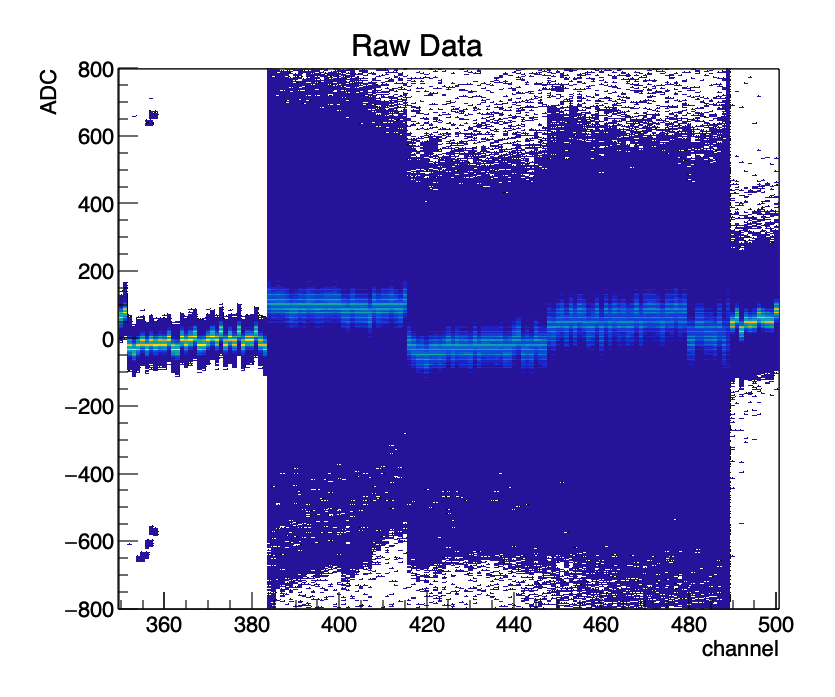
\includegraphics[width = 0.49\textwidth]{figures/raw_data.png} 
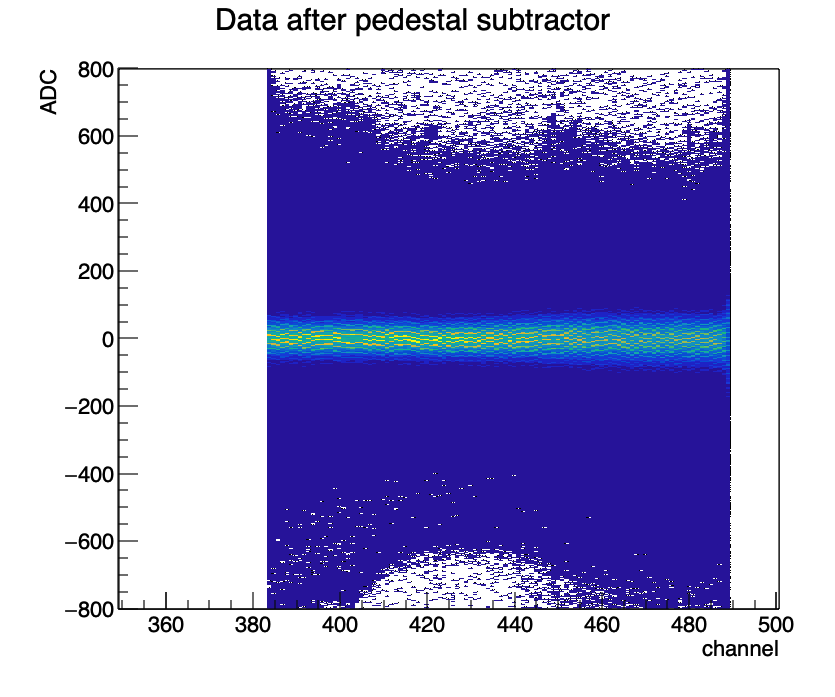
\includegraphics[width = 0.49\textwidth]{figures/pedestal_data.png}
\caption{Exemplary Pedestal Subtraction Algorithm's monitoring plots. Typical raw data ADC values (left), Pedestal subtracted ADC values
(right). The channels below 380 and above 480 were masked since they are not connected to any front-end chip.} 
\label{fig:raw vs ped}
 \end{center}
\end{figure}


\section{Common mode subtraction}
The next step within the TbUT processing chain is Common mode subtraction and the noise calculation. The noise, one floating-point number per channel,  is then used as a clustering threshold value for the clusterization algorithm described in the next section. 


The total noise affecting the signal measurement consists of two main components,  the first one affects every read-out channel independently, and the second one is common to the group of consecutive channels.  This type of noise is called Common Mode, and its origin can be grand loops in the power supplies, or read-out strips might pick some environmental noise. 

The Common Mode suppression algorithm consists of two phases. The first one was implemented to calculate the average pedestal-subtracted ADC value of the channels in 32-channel groups. This value is calculated for each event independently. Using this mean value, a search for particle hits is performed for each channel. All channels with hits are masked, and a new mean value is calculated for each 32-channel group. The channel is masked when its ADC value fulfills the following condition:

\begin{equation}
    |ADC_{i}(n)-CMS^{corr}_{i}| > \alpha \sigma^{RMS}_{i}
\end{equation}
where $\sigma^{RMS}_{i}$ is a channel ADC Root Mean Square, $CMS^{corr}_{i} $ is a correction for an event $i$, and $\alpha$ is a tunable parameter, that specifies the required distance between noise and signal. After the initial testbeam studies, this parameter was set to 4. 
The previously calculated mean value is then used to correct the ADC values in all channels of the 32-channel group.

The second phase of the CMS algorithm is calculation of the noise per channel, according to the following formula: 

\begin{equation}
    \sigma_i  = \sqrt{\frac{\sum_{n=1}^{N} (ADC_{i}(n)-\mu_{i})^2}{N}}
\end{equation}
where $\mu_{i} = \sum_{n=1}^{N} ADC_{i}(n)$ is a mean ADC value per channel. 


Figure \ref{fig:projections} presents the one-dimensional projection of the data after pedestal and Common Mode subtraction. It is clearly visible, based on the noise values, that the Common mode removal step is necessary to reduce the noise level and thus increase the Signal-to-Noise (S/N) ratio. 

A few typical events after all corrections applied are shown in figure \ref{fig:Noise}. Here, no requirement is made on the number of tracks. Strips with large ADC counts are indicative of the passage of a beam particle through the detector. The other channels show roughly Gaussian fluctuations about zero, typical of incoherent detector noise. Signals generally
stand out significantly above the noise. These examples were selected to visualize a couple of cases that may occur, such as double strip clusters (event 14) and multiple clusters per event (event 83).  


\begin{figure}[h]
  \centering
\begin{tabular}{c c}
\subfloat{{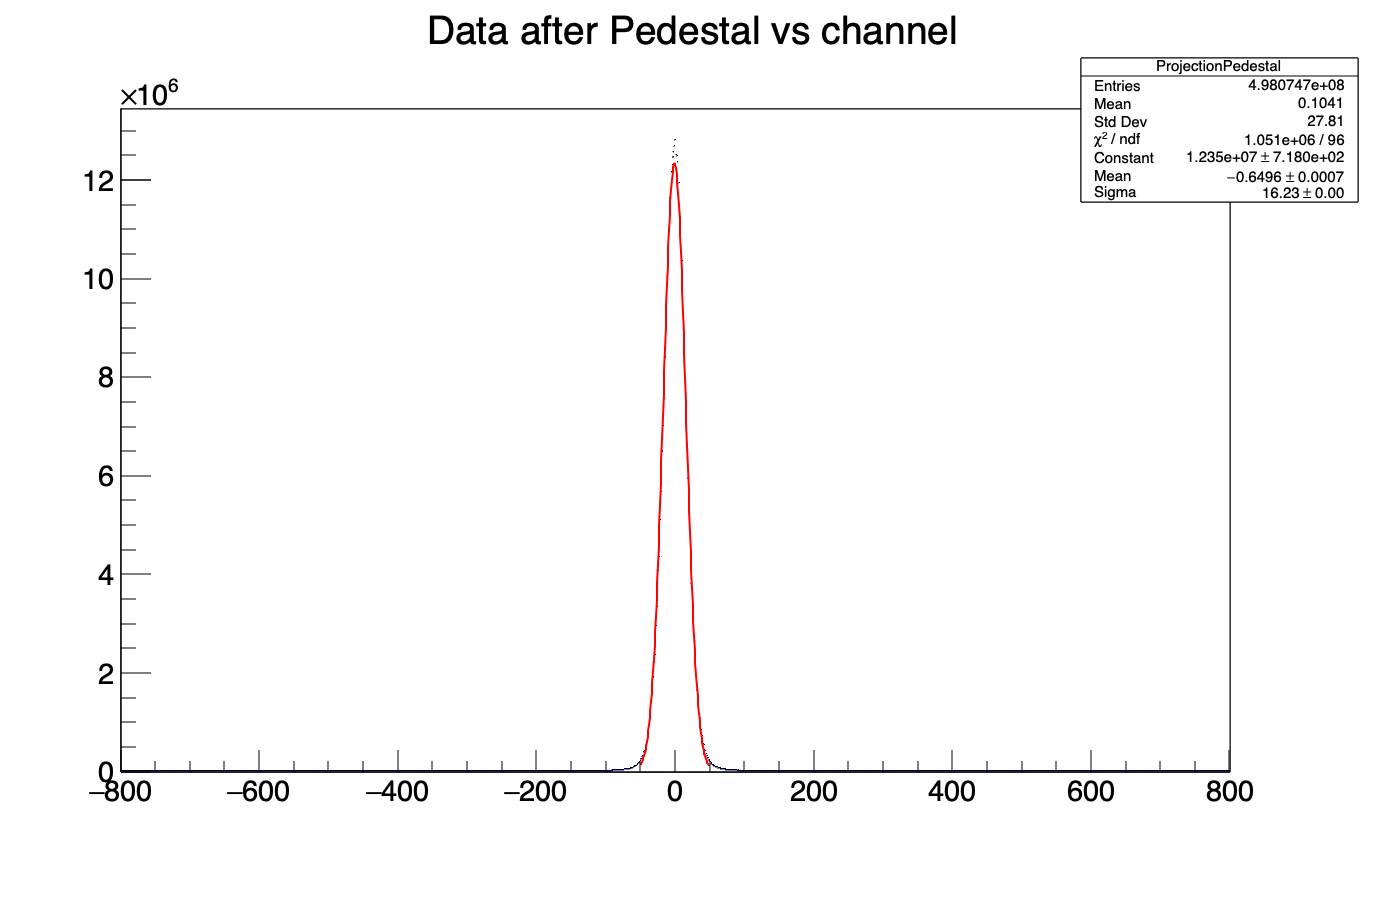
\includegraphics[width=0.5\textwidth]{figures/Pedestal_projection.png} }}%
    \subfloat{{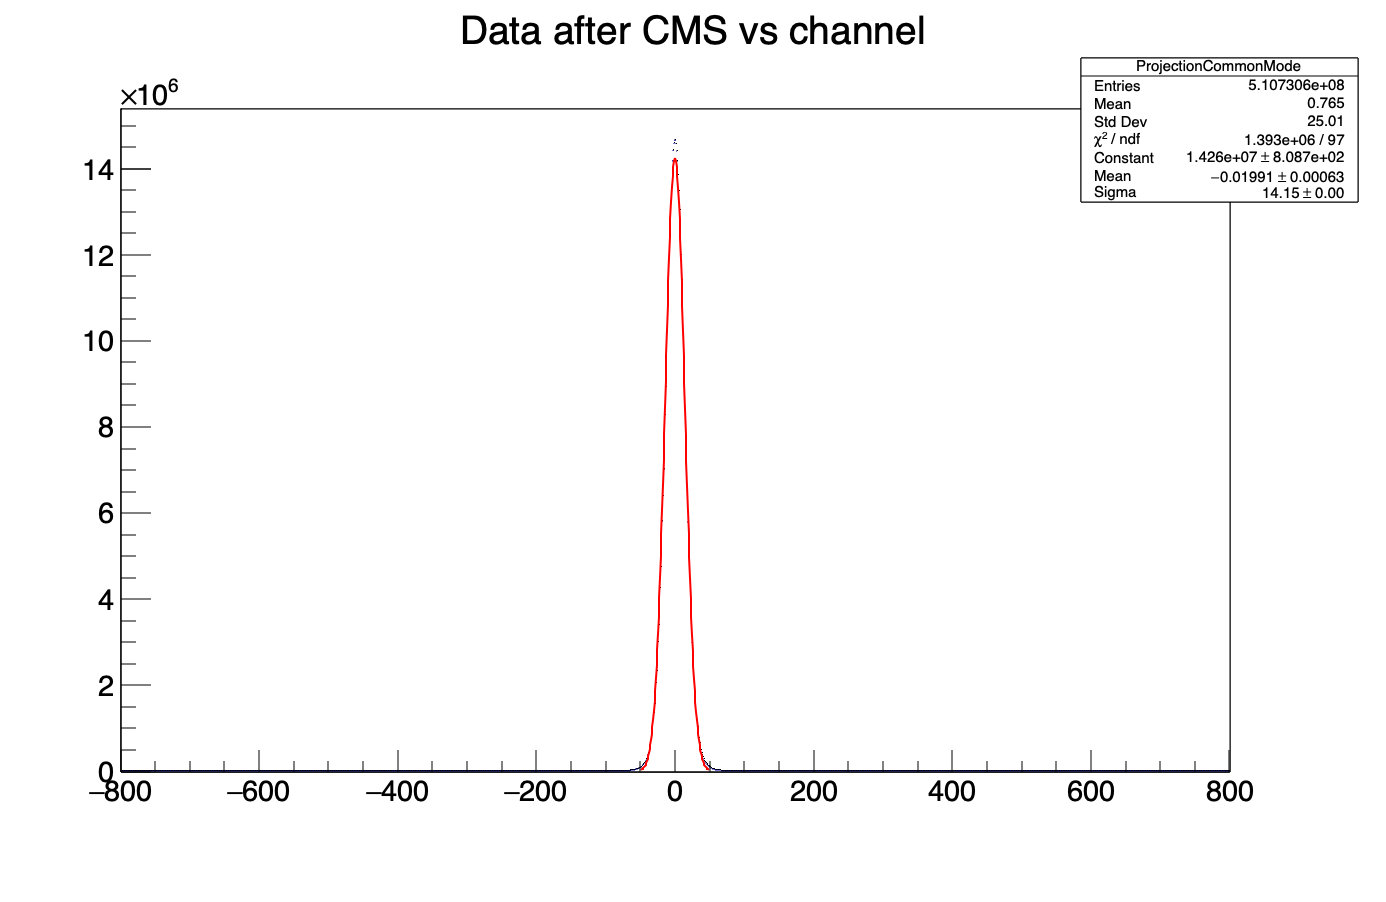
\includegraphics[width=0.5\textwidth]{figures/CMS_projection.png} }}%
\end{tabular}
   \caption{Projection of data after pedestal subtraction (left) and CMS (right)
\label{fig:projections}}  
\end{figure}

\begin{figure}[!h]
  \centering
\begin{tabular}{c c}
\subfloat{{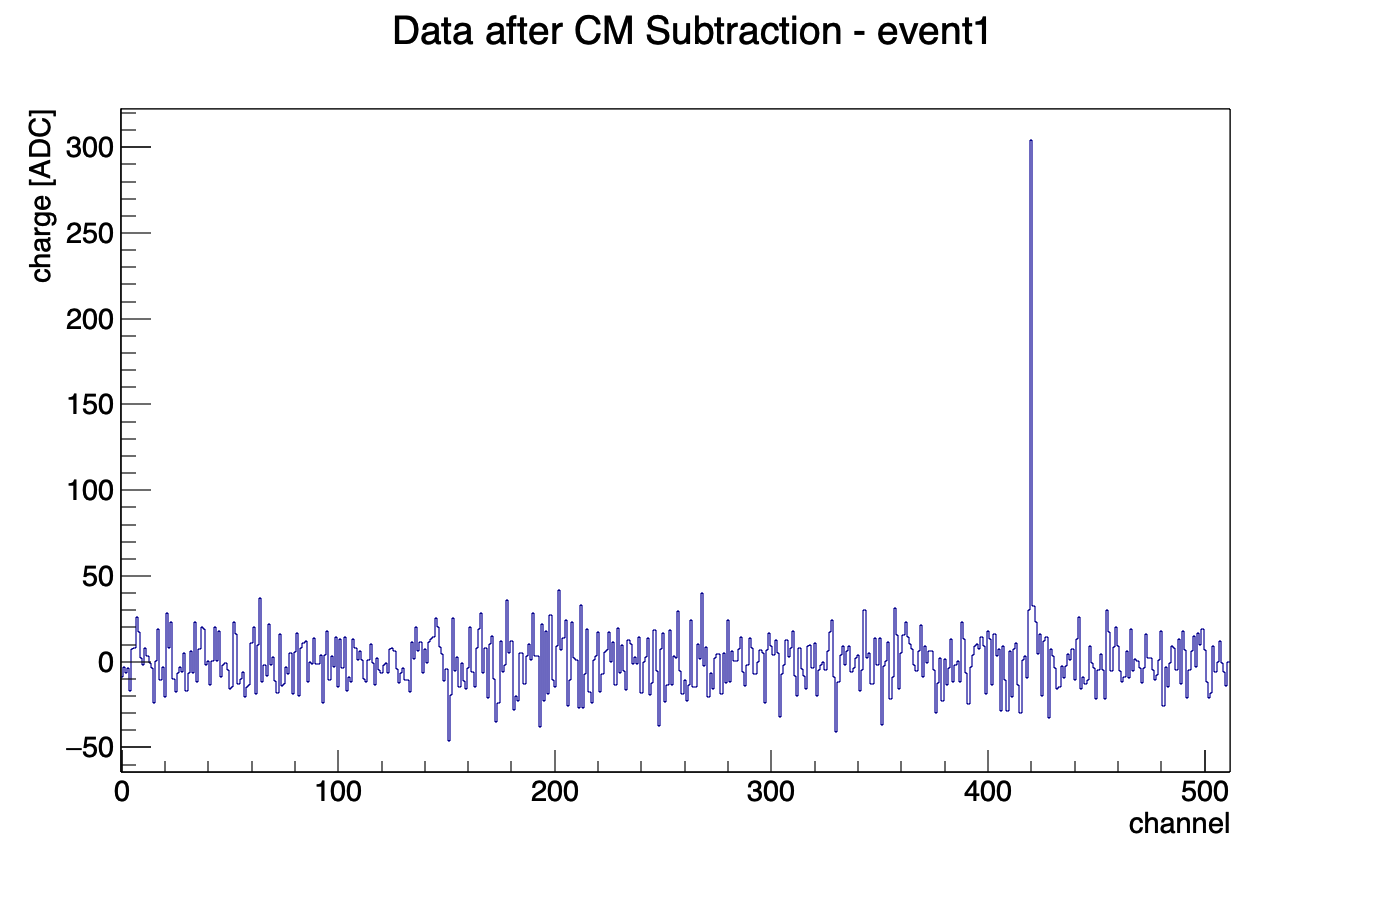
\includegraphics[width=0.5\textwidth]{figures/event1.png} }}%
    \subfloat{{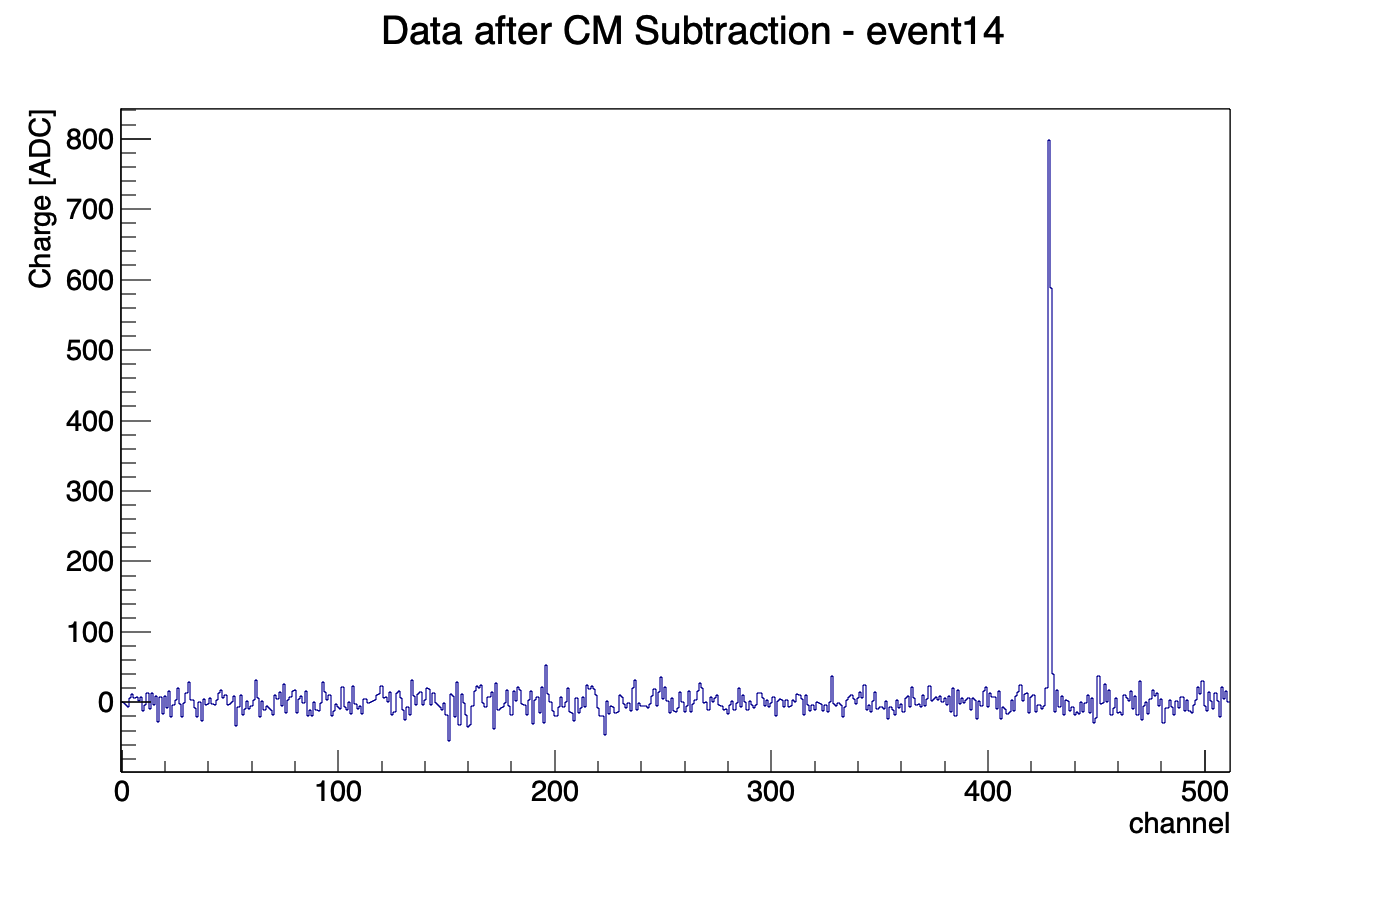
\includegraphics[width=0.5\textwidth]{figures/event2.png} }}%
\\
\subfloat{{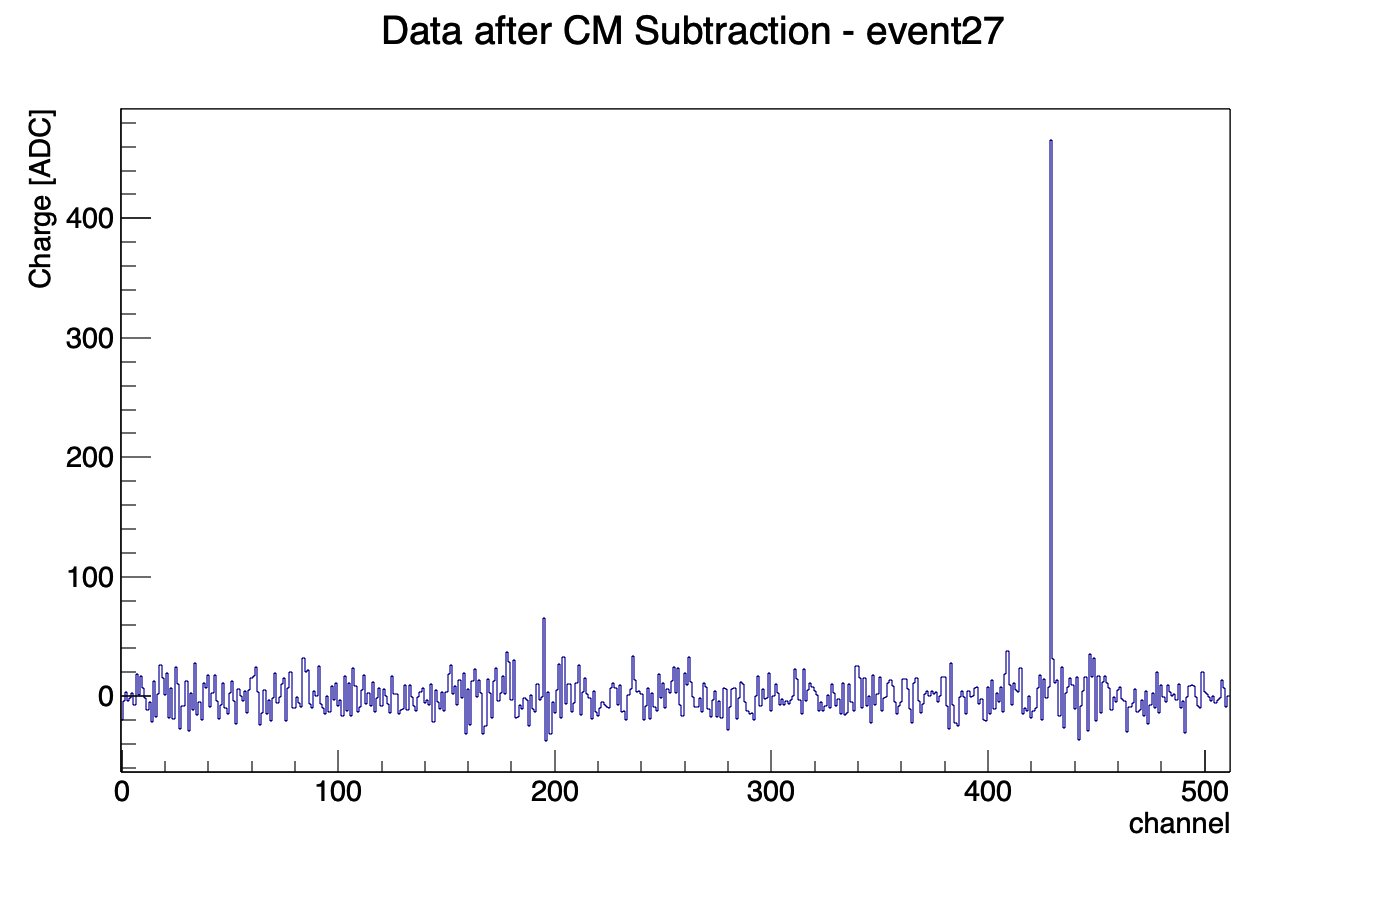
\includegraphics[width=0.5\textwidth]{figures/event3.png} }}%
    \subfloat{{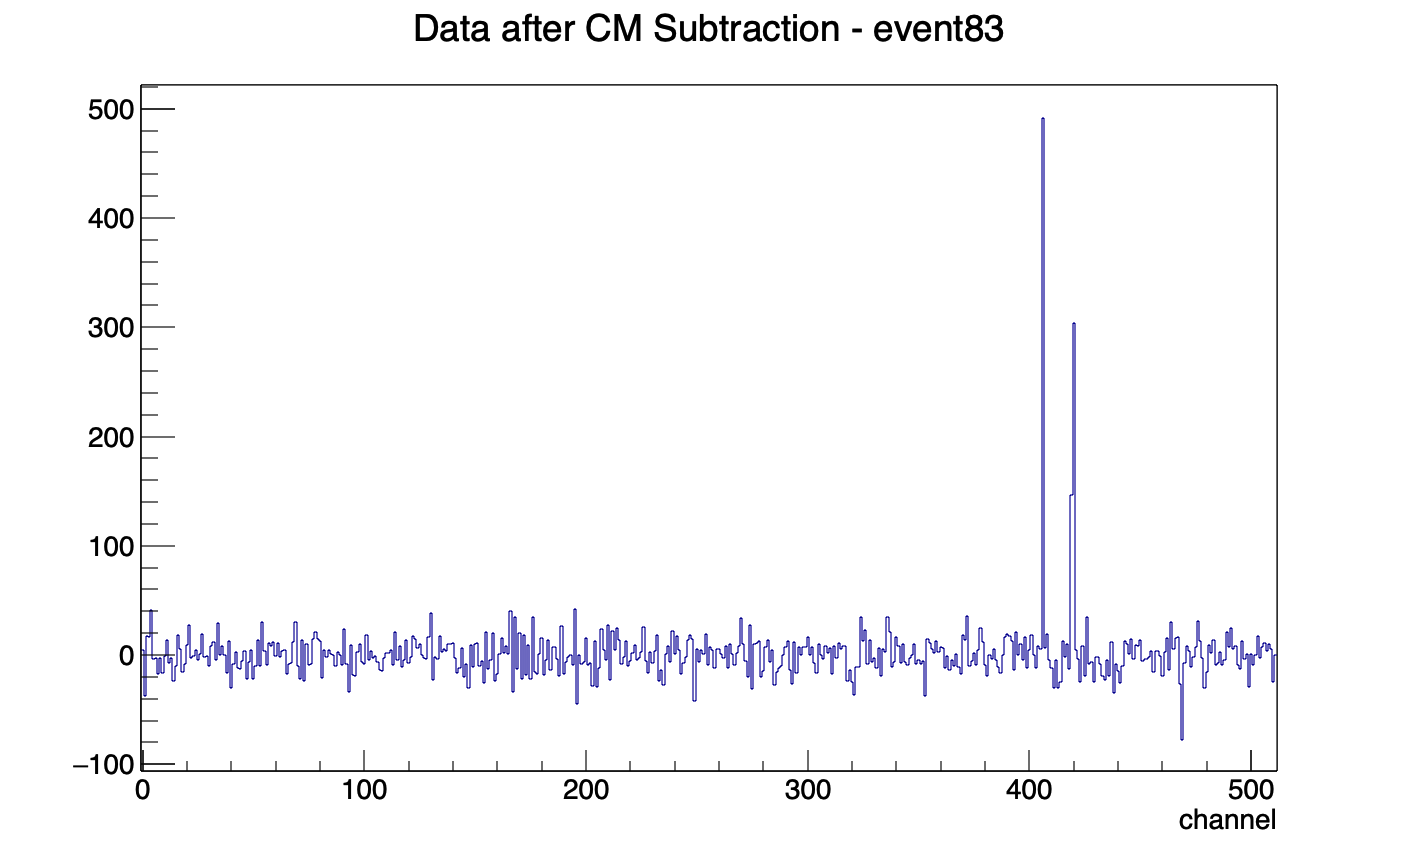
\includegraphics[width=0.5\textwidth]{figures/event4.png} }}%
\\
\subfloat{{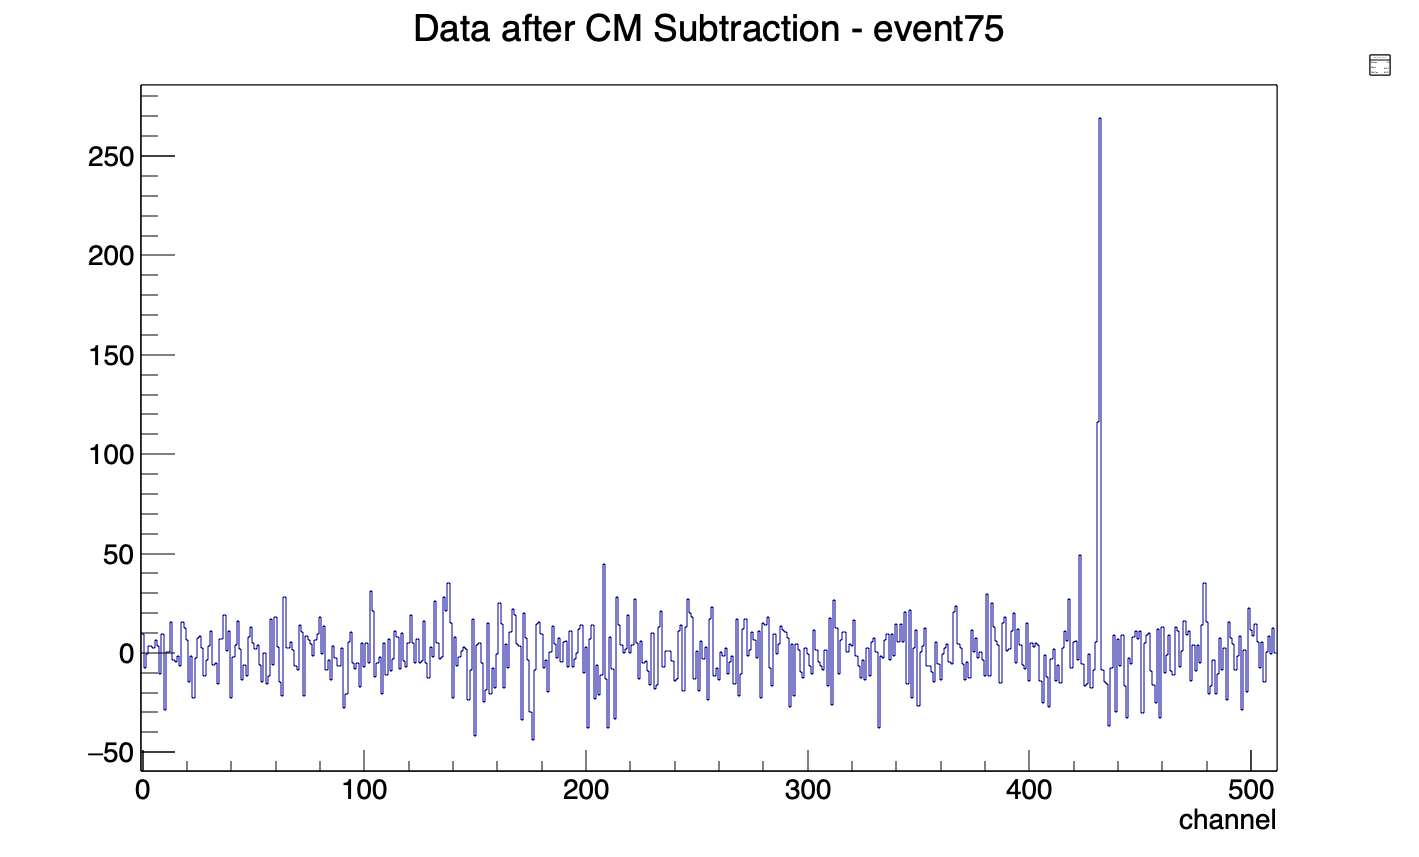
\includegraphics[width=0.5\textwidth]{figures/event5.png} }}%
    \subfloat{{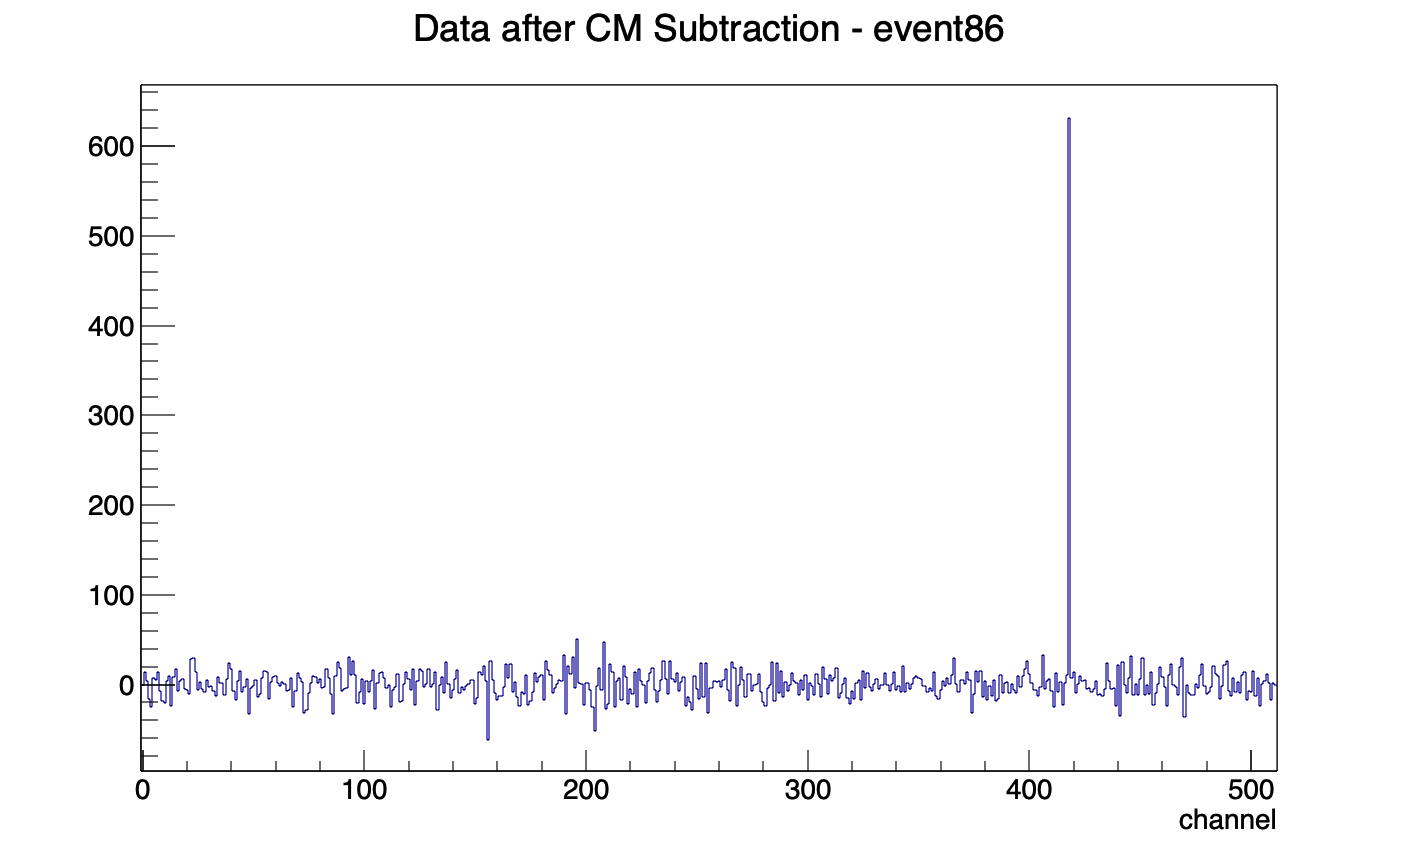
\includegraphics[width=0.5\textwidth]{figures/event6.png} }}%

\end{tabular}
   \caption{A few examples of a single events after pedestal and common mode removal.  
\label{fig:Noise}}  
\end{figure}




\begin{figure}[!h]
  \centering
\begin{tabular}{c c}
\subfloat{{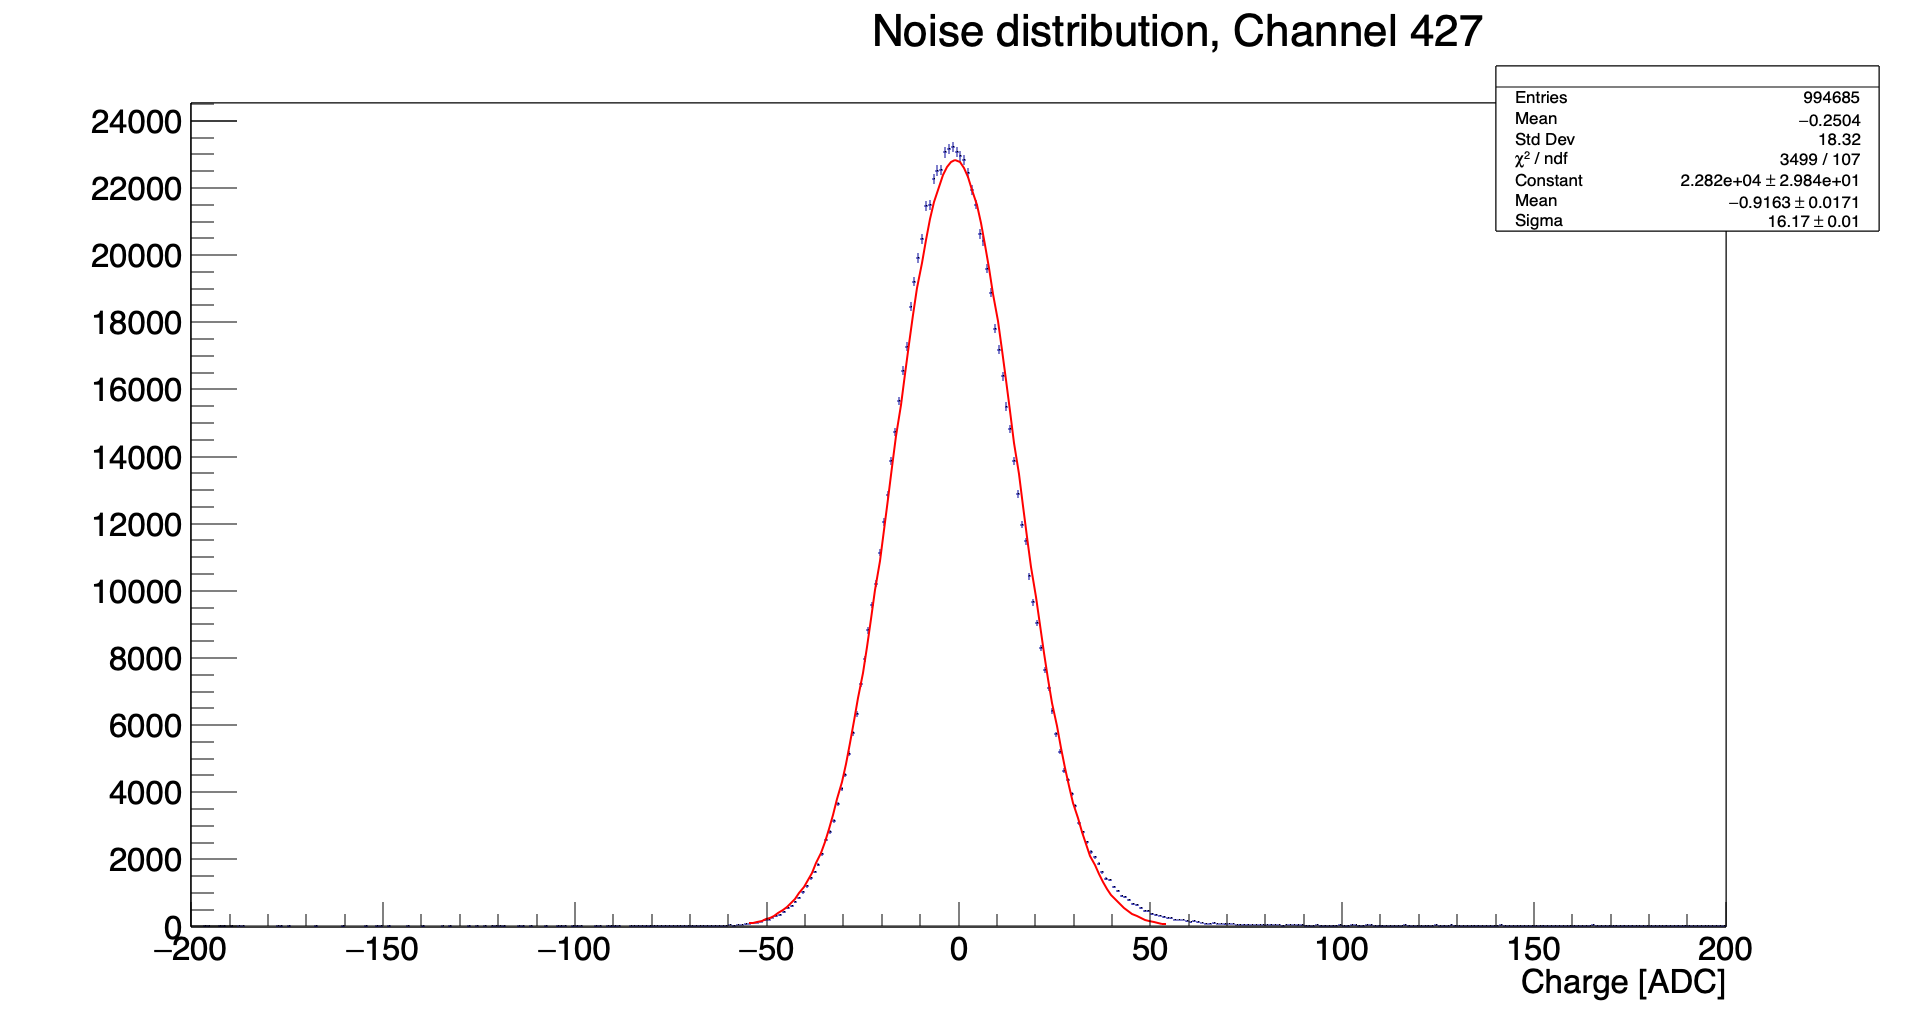
\includegraphics[width=0.5\textwidth]{figures/Noise2.png} }}%
    \subfloat{{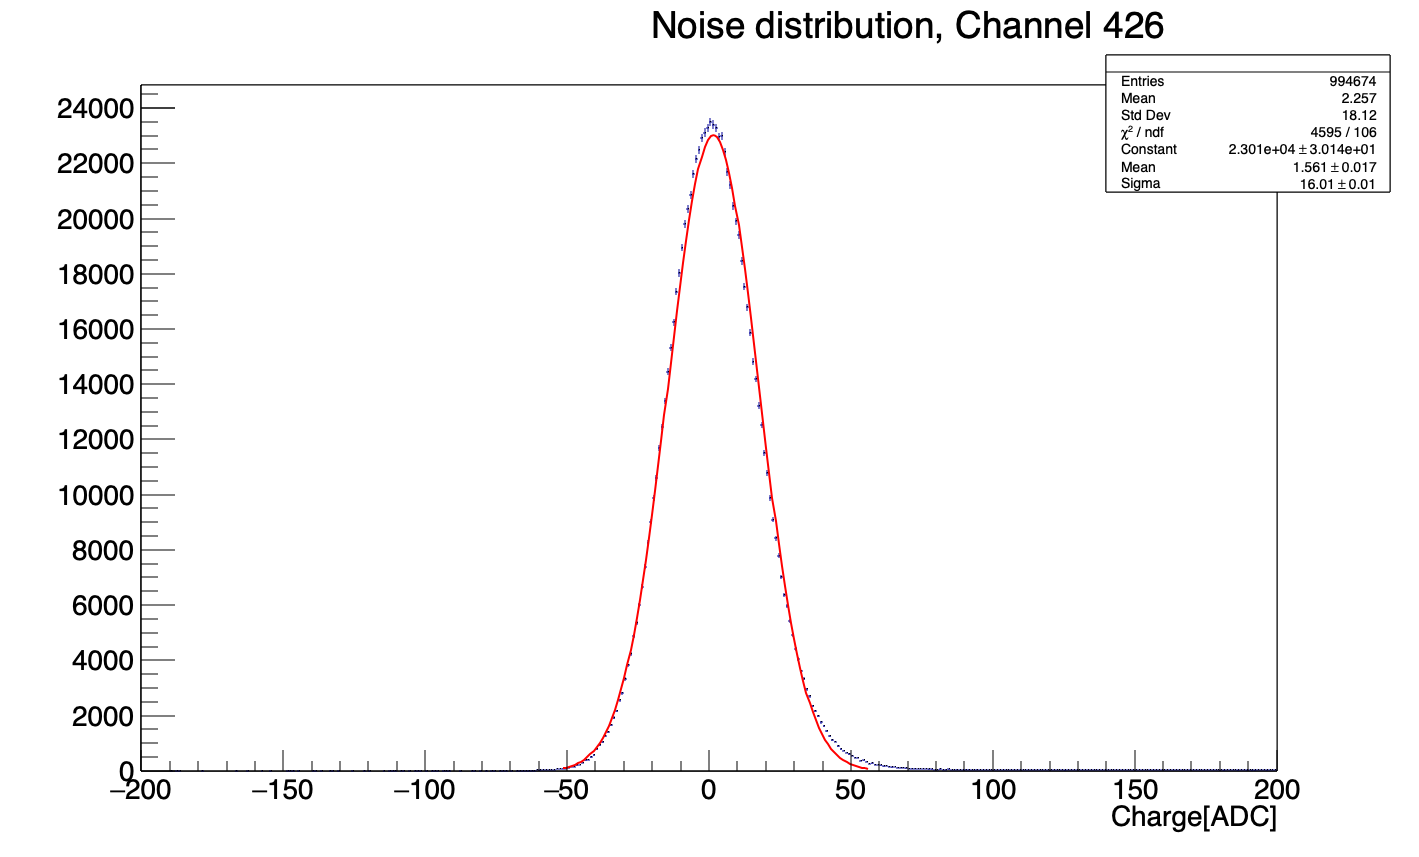
\includegraphics[width=0.5\textwidth]{figures/Noise0.png} }}%
\\
\subfloat{{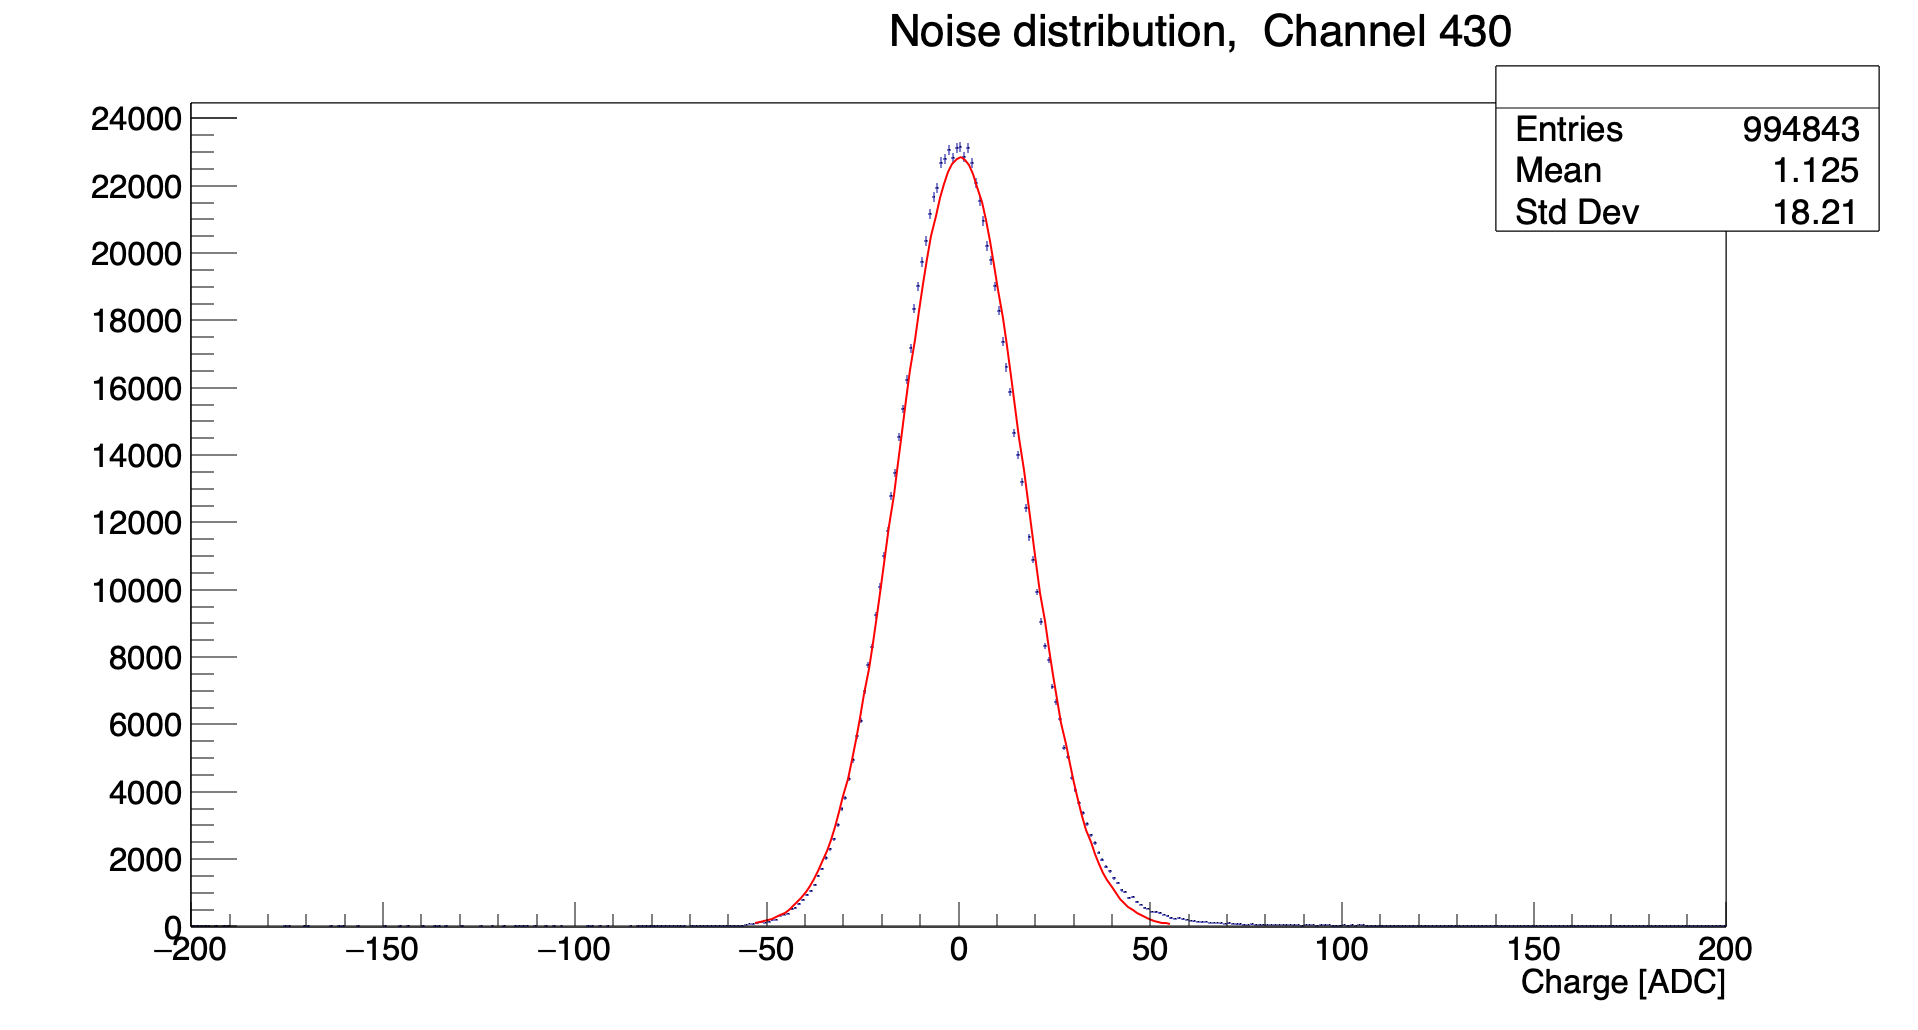
\includegraphics[width=0.5\textwidth]{figures/Noise3.png} }}%
    \subfloat{{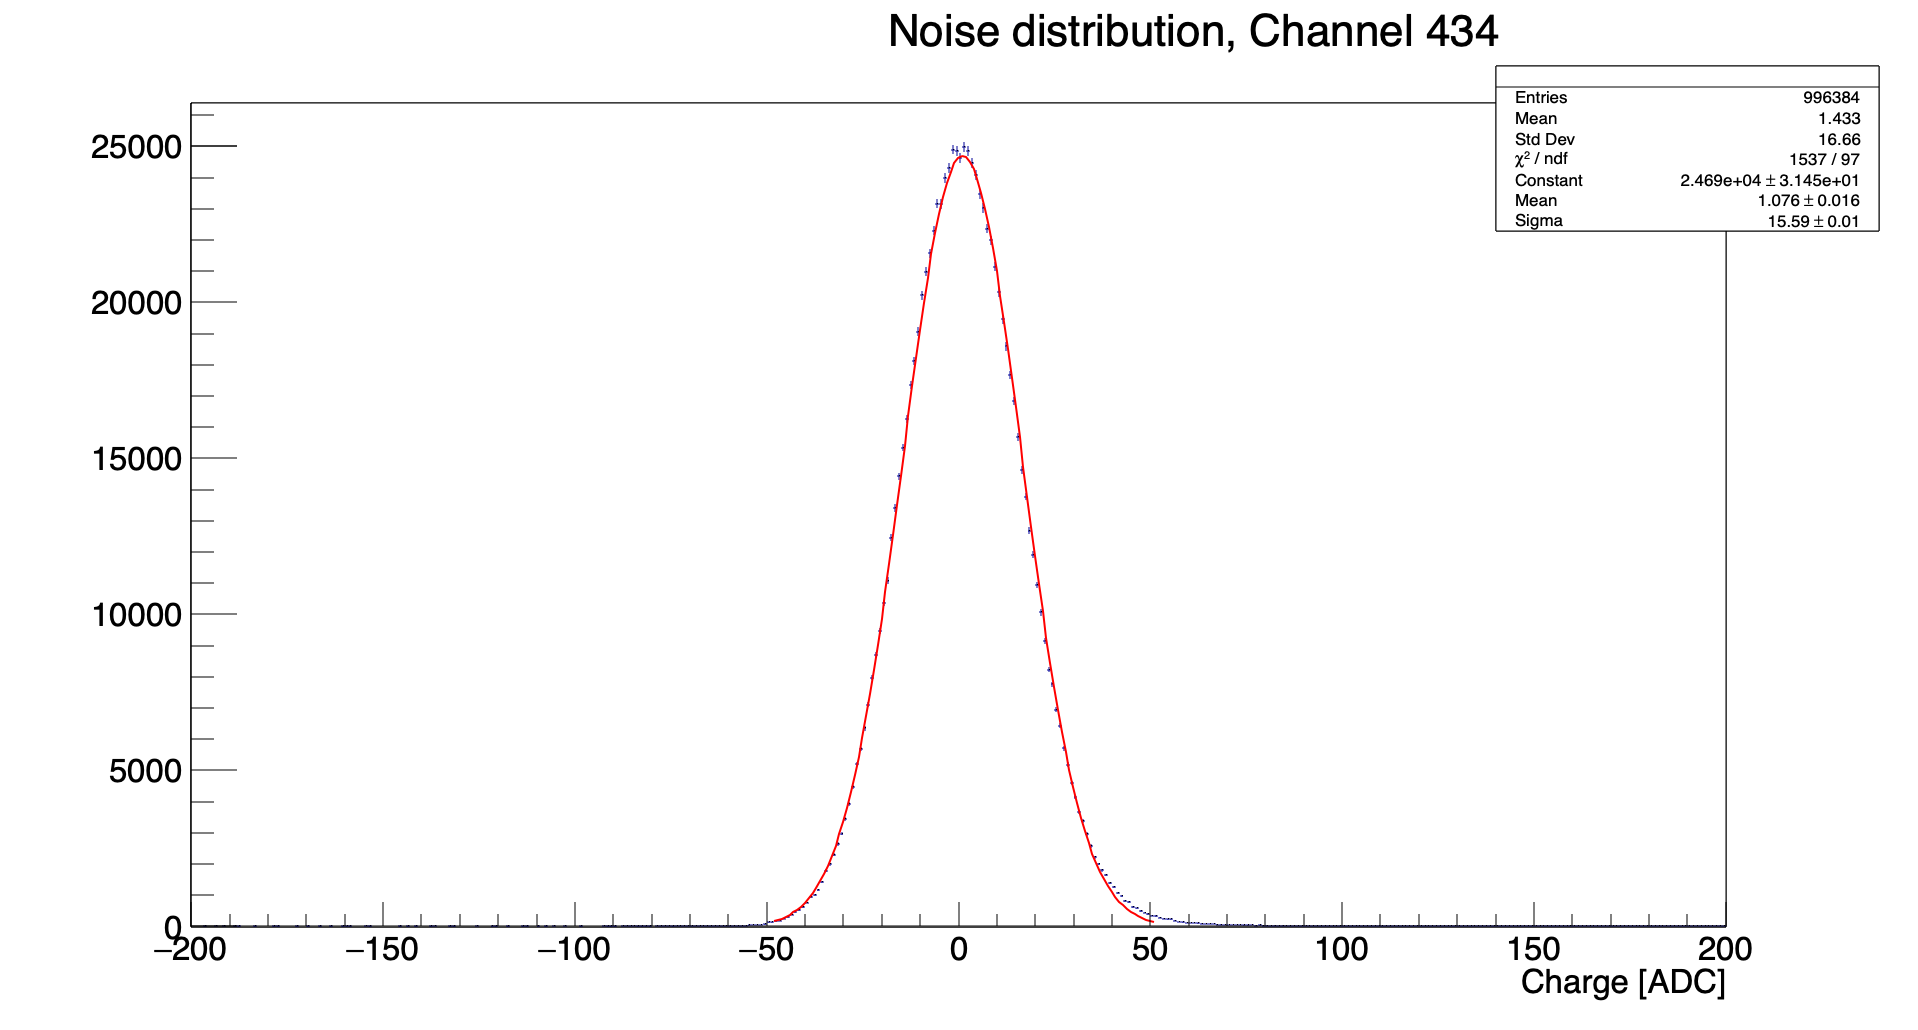
\includegraphics[width=0.5\textwidth]{figures/Noise4.png} }}%
\\
\subfloat{{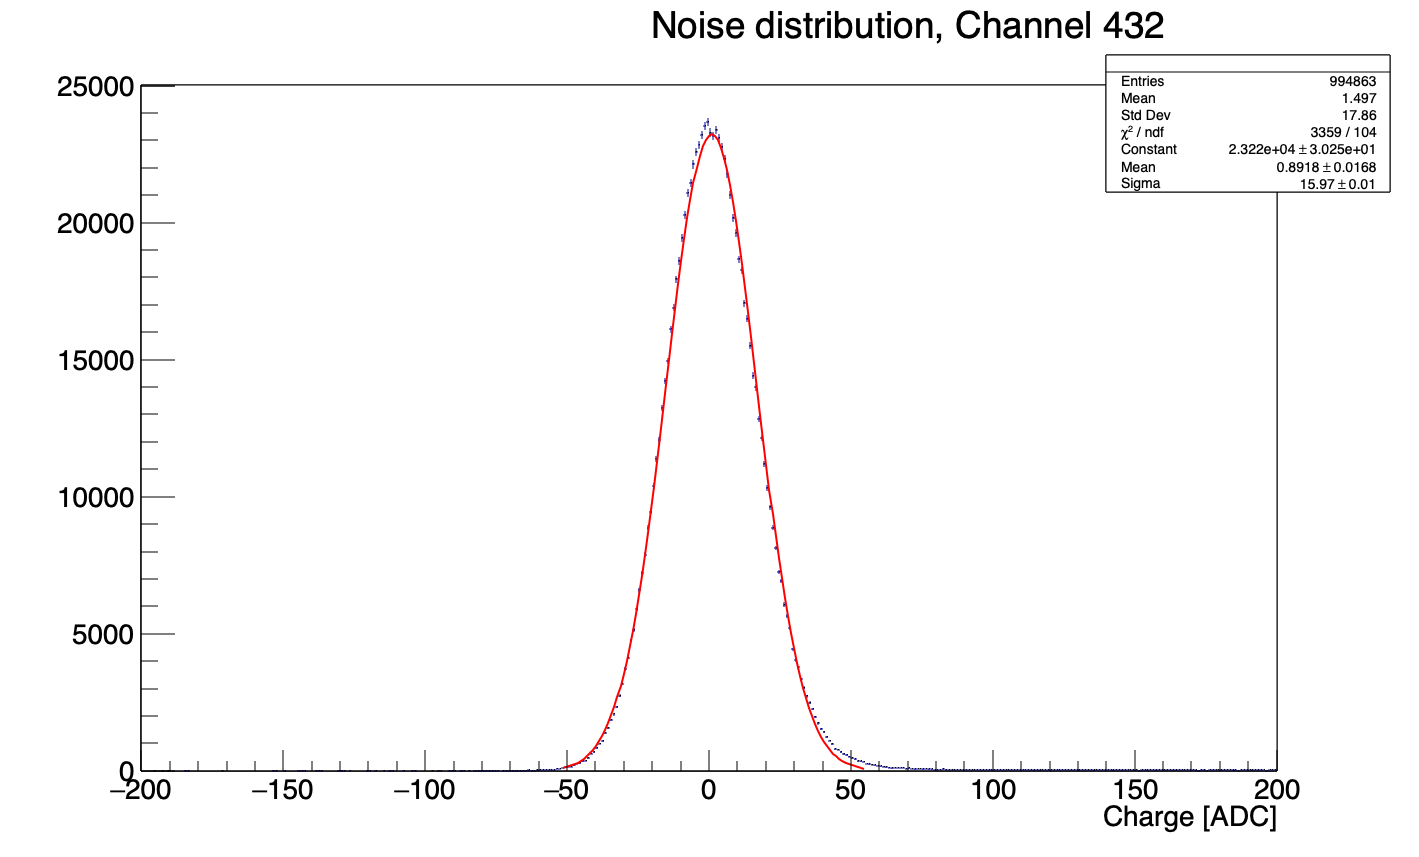
\includegraphics[width=0.5\textwidth]{figures/Noise5.png} }}%
    \subfloat{{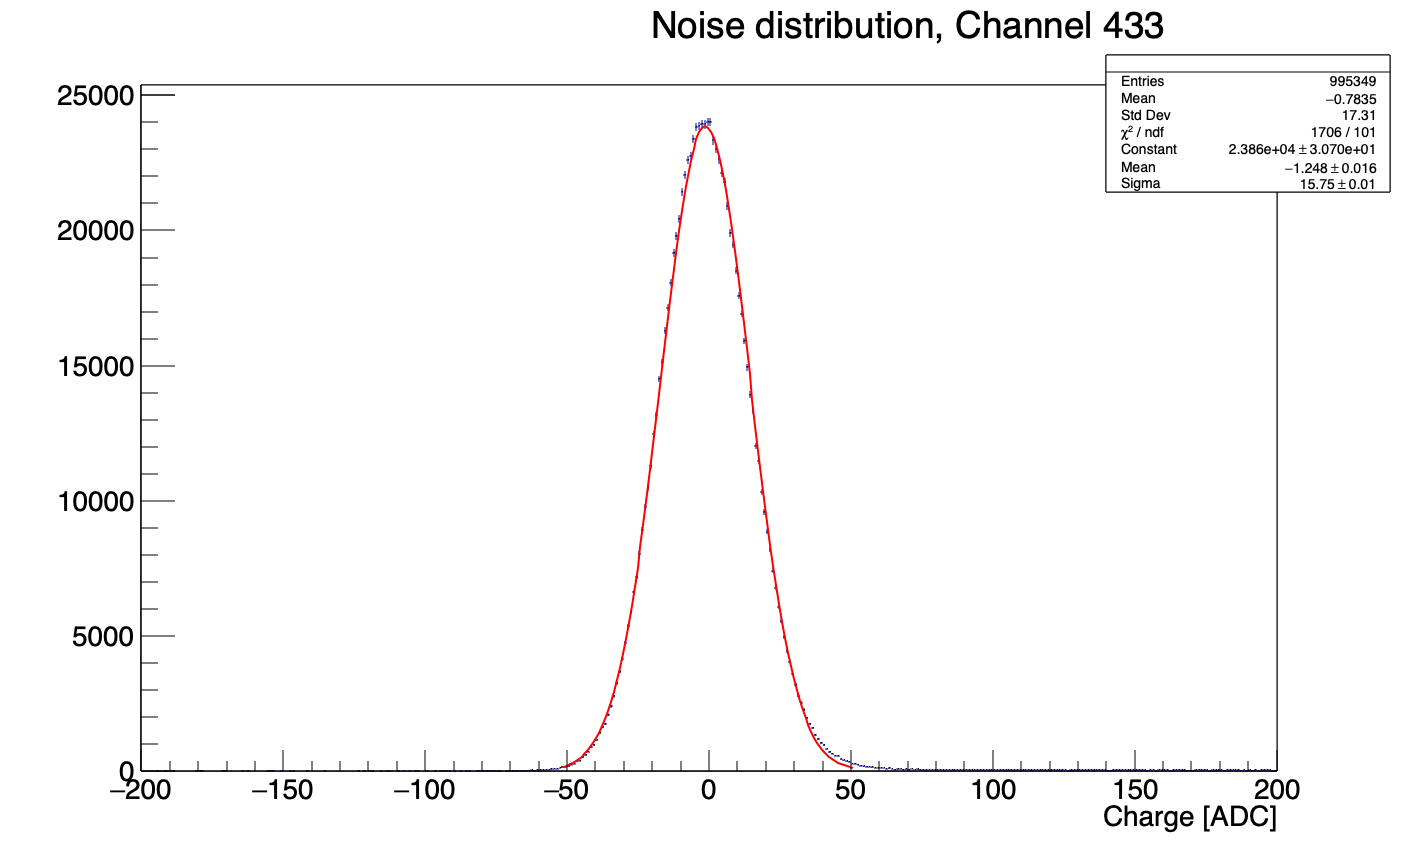
\includegraphics[width=0.5\textwidth]{figures/Noise6.png} }}%

\end{tabular}
   \caption{Noise distributions after Common Mode Suppression for selected channels within the beam region. The red curves show a Gaussian fit to the core of the distribution. 
\label{fig:Noise}}  
\end{figure}


\section{Cluster finding algorithm}

The final algorithm is executed to reconstruct a cluster using previously proceeded ADC values and noise per channel, which plays the role of the clusterization threshold.  
The additional algorithm's input parameters are the value of the low and high thresholds. 
Clusters in the DUT are built up by searching for a seed strip that has a collected charge more than a high threshold value. The outcome of this subroutine is a list of cluster seeds. The next subroutine is dedicated to removing the seeds that belong to the same clusters. Such a situation occurs when the cluster has more than one strip, and all of them have collected charges value higher than the high threshold. 
Moving away from the seed strip, the adjacent side strips having at least ADC count as low threshold are added to the cluster seed. The cluster is terminated when a side strip charge is below a low threshold. Thus, by definition, a cluster has between 1 and 5 strips included.
When there are multiple strips in the cluster, the position is computed using linear charge weighting:

\begin{equation}
    x_{cluster} = \frac{\sum^{S}_{i=1}x_i q_i}{{\sum_{i=1}{S}{q_i}}}
\end{equation}
where $x_i$ and $q_i$ are the positions and charges of
the strips in the cluster, and $S$ is the number of strips that constitute the cluster. 
\begin{algorithm}[caption={cluster creator algorithm}, label={al:cluster creator}]
Data: ADC data after Common Mode Suppression ($1 \ldots N$ events), clusterization thresholds (one floating-point number per channel)
Result: vector of reconstructed clusters

for event in $1 \ldots N$ do :
   find cluster seeds;
   remove seeds belonging to the same clusters;
   extend cluster seeds by adding adjacent strips;
   calculate cluster position
end
\end{algorithm}


The outcome of the clusterization algorithm can be used to visualize the quality of the collected data. One of the most important plots is a histogram presenting the distribution of the cluster charge. To get physics quantities describing the sensor's performance, the cluster charge data is fitted with the Landau Gauss convolution model. The parameter of this fit allows determining the Most Provable Value and the width of the signal.  Figure \ref{fig:clusters_with_landau} presents a collection of cluster charge distribution histograms. Those histograms were created on top of the data collected during the one of the testbeam. They were used to show the sensor performance versus the bias voltage applied to them.  Those studies were conducted to investigate the effect of a drop in the collected charge when sensor irradiation increases, which was seen previously \cite{irradiation}. The collected charge drop may lead to decreasing the Signal to Noise ratio.  


\begin{figure}
\centering
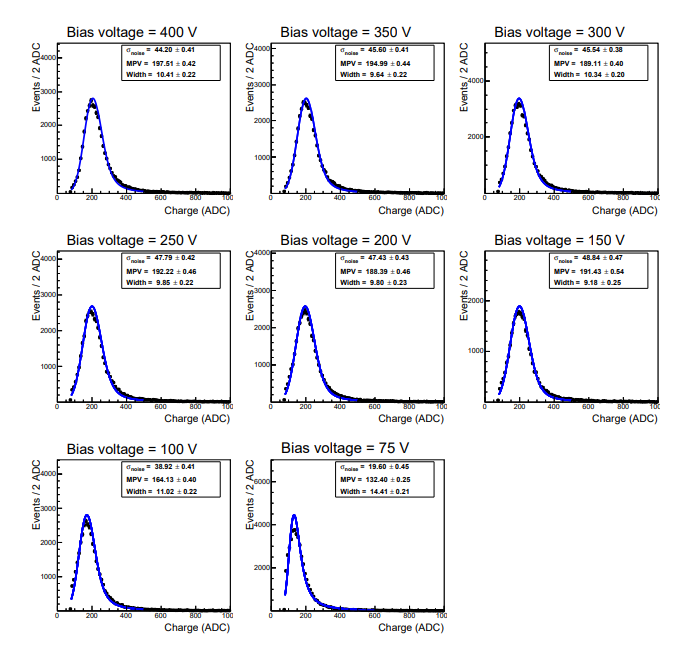
\includegraphics{figures/landau.png}
\caption{Cluster charge distributions. The data are fit to a Landau 
convoluted with a Gaussian resolution function, and the fit is shown (solid blue line). Figures taken from \cite{tb1}. 
}\label{fig:clusters_with_landau}
\end{figure}

The second type of monitoring plot is a distribution of cluster size. That plot allows better understanding of how the resolution of the sensors changes as a function of the angle between the incident particle and the normal to the sensor. Figure \ref{fig:clusters_size} presents a cluster size as a function of the sensor rotation angle obtained using data collected during the 2015 testbeam. 


\begin{figure}
\centering
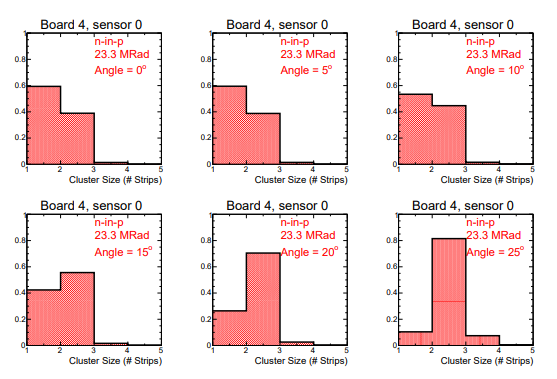
\includegraphics{figures/Cluster_size.PNG}
\caption{Cluster size distributions. Figures taken from \cite{tb1}. 
}\label{fig:clusters_size}
\end{figure}

 